% Thesis Figure 6.1: architecture of the SAFAIR adversarial benchmark tool, redrawn after
% D7.6 Figure 2 (printed p. 22, PDF p. 29); the original raster stays in
% ../sparta/report-originals/d76-fig02-benchmark-architecture.jpg.
% Box labels follow the original figure, with scikit-learn in its own spelling. The second
% line in each box paraphrases D7.6 Section 3.1.1: the five modules, the setup files that
% select attacks, datasets and use cases, and the run that attacks a trained model and
% reports task-dependent output (D7.6 Figures 4-6).
% Geometry is in millimetres with y pointing down; 140 mm fits the text block at 1:1.
\documentclass[border=1pt]{standalone}
% Shared typography and palette for the three corrected SWaT context figures.
% Geometry is in millimetres; 140 mm fits the thesis text block at native scale.
\usepackage[T1]{fontenc}
\usepackage{tgheros}
\renewcommand{\familydefault}{\sfdefault}
\usepackage{tikz}
\usetikzlibrary{calc,patterns}
\definecolor{swatblue}{HTML}{0065BD}
\definecolor{swatlight}{HTML}{98C6EA}
\definecolor{swatgrey}{HTML}{666666}
\tikzset{every node/.style={font=\fontsize{8}{10}\selectfont},
  panel/.style={draw=black!30,fill=white,line width=0.4pt},
  stage/.style={draw=swatblue,fill=swatblue,text=white,align=center,
    minimum height=10mm,text width=19mm,inner sep=0.5mm},
  smalllabel/.style={font=\fontsize{7}{8.5}\selectfont,text=swatgrey}}

\usetikzlibrary{arrows.meta}
\newcommand{\fT}{\fontsize{7.5}{9}\selectfont\bfseries}
\newcommand{\fH}{\fontsize{7}{8.4}\selectfont\bfseries}
\newcommand{\fB}{\fontsize{7}{8.4}\selectfont\mdseries}
\newcommand{\fX}{\fontsize{6}{7.2}\selectfont\mdseries}
% Five rows of 10.5 mm boxes on a 13 mm pitch, starting 7 mm below the panel top.
\def\BH{10.5}\def\PITCH{13}\def\HT{72.5}
\newcommand{\rowy}[1]{%
  \pgfmathsetmacro{\yt}{7+\PITCH*#1}%
  \pgfmathsetmacro{\yb}{\yt+\BH}%
  \pgfmathsetmacro{\yc}{\yt+\BH/2}}
% Third-party library: row, name, kind.
\newcommand{\libbox}[3]{\rowy{#1}%
  \draw[op] (1.5,\yt) rectangle (38.5,\yb);
  \node[txt,align=center] at (20,\yc) {{\fB #2}\\[0.35mm]{\fX\color{swatgrey}#3}};}
% Benchmark module: row, name, role.
\newcommand{\modbox}[3]{\rowy{#1}%
  \fill[swatblue] (51.5,\yt) rectangle (88.5,\yb);
  \node[txt,align=center,text=white] at (70,\yc) {{\fH #2}\\[0.35mm]{\fX #3}};}
% Run-time step: row, box style, label, note.
\newcommand{\runbox}[4]{\rowy{#1}%
  \draw[#2] (101.5,\yt) rectangle (138.5,\yb);
  \node[txt,align=center] at (120,\yc) {{#3}\\[0.35mm]{\fX\color{swatgrey}#4}};}
\begin{document}
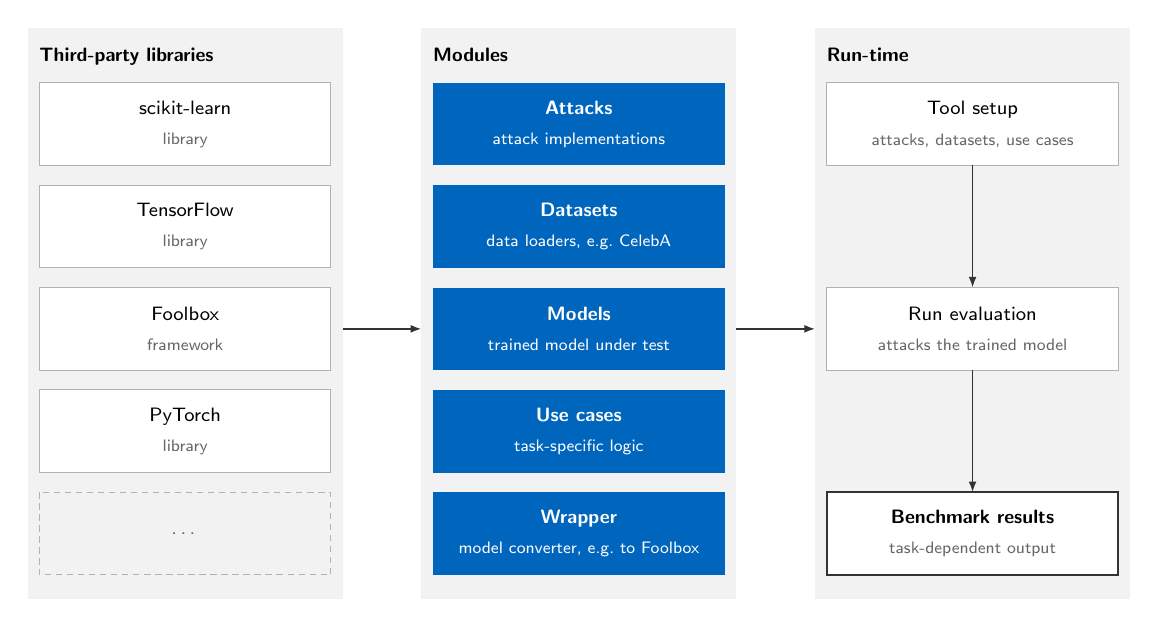
\begin{tikzpicture}[x=1mm,y=-1mm,
    txt/.style={inner sep=0pt,outer sep=0pt},
    op/.style={draw=black!30,fill=white,line width=0.4pt},
    outbox/.style={draw=black!80,fill=white,line width=0.6pt},
    lnk/.style={draw=black!80,line width=0.6pt},
    arr/.style={lnk,-{Latex[length=1.35mm,width=1mm]}}]
  \path[use as bounding box] (0,0) rectangle (140,\HT);

  % Panels
  \fill[black!5] (0,0) rectangle (40,\HT);
  \fill[black!5] (50,0) rectangle (90,\HT);
  \fill[black!5] (100,0) rectangle (140,\HT);
  \node[txt,anchor=base west] at (1.5,4.3) {\fT Third-party libraries};
  \node[txt,anchor=base west] at (51.5,4.3) {\fT Modules};
  \node[txt,anchor=base west] at (101.5,4.3) {\fT Run-time};

  % Third-party libraries; the dashed slot stands for the original's ellipsis
  \libbox{0}{scikit-learn}{library}
  \libbox{1}{TensorFlow}{library}
  \libbox{2}{Foolbox}{framework}
  \libbox{3}{PyTorch}{library}
  \rowy{4}
  \draw[black!30,line width=0.4pt,dash pattern=on 0.8mm off 0.6mm]
    (1.5,\yt) rectangle (38.5,\yb);
  \node[txt,text=swatgrey] at (20,\yc) {\fB\dots};

  % Modules
  \modbox{0}{Attacks}{attack implementations}
  \modbox{1}{Datasets}{data loaders, e.g.\ CelebA}
  \modbox{2}{Models}{trained model under test}
  \modbox{3}{Use cases}{task-specific logic}
  \modbox{4}{Wrapper}{model converter, e.g.\ to Foolbox}

  % Run-time
  \runbox{0}{op}{\fB Tool setup}{attacks, datasets, use cases}
  \runbox{2}{op}{\fB Run evaluation}{attacks the trained model}
  \runbox{4}{outbox}{\fH Benchmark results}{task-dependent output}
  \rowy{0}\let\ya\yb \rowy{2}\let\yd\yt \let\ye\yb \rowy{4}\let\yf\yt
  \draw[arr] (120,\ya) -- (120,\yd);
  \draw[arr] (120,\ye) -- (120,\yf);

  % Group dependencies
  \rowy{2}
  \draw[arr] (40,\yc) -- (50,\yc);
  \draw[arr] (90,\yc) -- (100,\yc);
\end{tikzpicture}
\end{document}
